% Chapter Template

\chapter{STUDY OF VMWALL\citep{Reference2}} % Main chapter title

\label{Chapter4} % Change X to a consecutive number; for referencing this chapter elsewhere, use \ref{ChapterX}

\lhead{Chapter X. \emph{STUDY OF VMWALL}} % Change X to a consecutive number; this is for the header on each page - perhaps a shortened title

Our strategy to achieve our goal is firstly to absorb inspiration from already-existing VMI applications. Among all the
VMI applications that we have studied, VMWall is relatively much closer to our design goal. This system implements
an application-level firewall working in Xen hypervisor. To achieve this, it needs to correlate each monitored TCP or
UDP connection with process which creates it. Although VMWall is implemented in Xen hypervisor and its source code
is not accessible, its work about how to correlate network traffic and corresponding process may give us some clues.

VMWall consists of two parts: user agent and kernel component. Kernel component uses a modified ebtables [21]
packet filter to intercept all packets sent to or from a guest domain. To well understand VMWall’s kernel component
implementation, it is supposed to be familiar with Xen network virtualization. In fact, Xen offers several different
9networking modes. VMWall uniquely considers the bridging mode. With this mode, Dom0 provides a virtual Ethernet
bridge connecting the physical network card to all virtual network devices provided by Xen to the domU VMs. Dom0
uses its virtual bridge to multiplex and demultiplex packets between the physical network interface and each
unprivileged virtual machine’s VNI (Virtual Network Interface). Due to this fact mentioned, kernel component (in this
case Ebtables) could intercept all packets between monitored VM and external Internet and retrieve information like IP
address and TCP/UPD port to identify a network connection.

If necessary, user agent, another important part of VMWall, will receive a request containing IP address and TCP ports
information and need to use the latter to identify the corresponding process running in monitored guest by out-of-band
pattern VMI. The correlation between network connection and process relies on one file type in Linux/Unix: socket.
Socket is a special file type in Linux/Unix world. To create a socket connection, IP address and transport layer port are
required. All opening port numbers in Linux are hashed and managed by data structure \lq inet\_hashinfo \rq. By iterating this
variable (for example tcp\_hashinfo) of this data structure, the socket file using a given port number could be identified. Similarly, all processes in Linux are managed by a double linked data structure \lq task\_struct \rq. With input of a certain socket reference, the process creating this socket could be found. The following picture shows how to correlate network
connection and process on data structure level.

\begin{figure}[htbp]
	\centering
		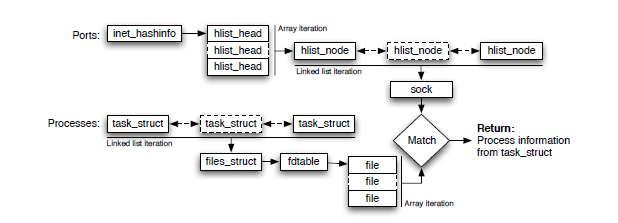
\includegraphics[scale = 0.8 ]{Figures/Figure4.png}
		% \rule{35em}{0.5pt}
	\caption[Out-of-Band pattern VMI applications]{Out-of-Band pattern VMI applications}
	\label{fig:Guest Linux kernel data structures traversed by the VMWall user agent during correlation of the
process and TCP packet information}
\end{figure}

%----------------------------------------------------------------------------------------
%	SECTION 1
%----------------------------------------------------------------------------------------

\section{Main Section 1}

Lorem ipsum dolor sit amet, consectetur adipiscing elit. Aliquam ultricies lacinia euismod. Nam tempus risus in dolor rhoncus in interdum enim tincidunt. Donec vel nunc neque. In condimentum ullamcorper quam non consequat. Fusce sagittis tempor feugiat. Fusce magna erat, molestie eu convallis ut, tempus sed arcu. Quisque molestie, ante a tincidunt ullamcorper, sapien enim dignissim lacus, in semper nibh erat lobortis purus. Integer dapibus ligula ac risus convallis pellentesque.

%-----------------------------------
%	SUBSECTION 1
%-----------------------------------
\subsection{Subsection 1}

Nunc posuere quam at lectus tristique eu ultrices augue venenatis. Vestibulum ante ipsum primis in faucibus orci luctus et ultrices posuere cubilia Curae; Aliquam erat volutpat. Vivamus sodales tortor eget quam adipiscing in vulputate ante ullamcorper. Sed eros ante, lacinia et sollicitudin et, aliquam sit amet augue. In hac habitasse platea dictumst.

%-----------------------------------
%	SUBSECTION 2
%-----------------------------------

\subsection{Subsection 2}
Morbi rutrum odio eget arcu adipiscing sodales. Aenean et purus a est pulvinar pellentesque. Cras in elit neque, quis varius elit. Phasellus fringilla, nibh eu tempus venenatis, dolor elit posuere quam, quis adipiscing urna leo nec orci. Sed nec nulla auctor odio aliquet consequat. Ut nec nulla in ante ullamcorper aliquam at sed dolor. Phasellus fermentum magna in augue gravida cursus. Cras sed pretium lorem. Pellentesque eget ornare odio. Proin accumsan, massa viverra cursus pharetra, ipsum nisi lobortis velit, a malesuada dolor lorem eu neque.

%----------------------------------------------------------------------------------------
%	SECTION 2
%----------------------------------------------------------------------------------------

\section{Main Section 2}

Sed ullamcorper quam eu nisl interdum at interdum enim egestas. Aliquam placerat justo sed lectus lobortis ut porta nisl porttitor. Vestibulum mi dolor, lacinia molestie gravida at, tempus vitae ligula. Donec eget quam sapien, in viverra eros. Donec pellentesque justo a massa fringilla non vestibulum metus vestibulum. Vestibulum in orci quis felis tempor lacinia. Vivamus ornare ultrices facilisis. Ut hendrerit volutpat vulputate. Morbi condimentum venenatis augue, id porta ipsum vulputate in. Curabitur luctus tempus justo. Vestibulum risus lectus, adipiscing nec condimentum quis, condimentum nec nisl. Aliquam dictum sagittis velit sed iaculis. Morbi tristique augue sit amet nulla pulvinar id facilisis ligula mollis. Nam elit libero, tincidunt ut aliquam at, molestie in quam. Aenean rhoncus vehicula hendrerit.